\documentclass[aspectratio=169]{beamer}
\usetheme{Madrid}
\usecolortheme{default}

\usepackage[utf8]{inputenc}
\usepackage{listings}
\usepackage{xcolor}
\usepackage{tikz}
\usepackage{graphicx}
\graphicspath{{./images/}}
\usetikzlibrary{positioning,shapes,arrows,calc,trees}

% Python code configuration
\lstset{
    language=Python,
    basicstyle=\ttfamily\tiny,
    keywordstyle=\color{blue},
    commentstyle=\color{green!60!black},
    stringstyle=\color{red},
    showstringspaces=false,
    breaklines=true,
    frame=single,
    numbers=left,
    numberstyle=\tiny\color{gray}
}

\title{Classification - Part 1}
\subtitle{K-Nearest Neighbors and Decision Trees}
\author{Meyssem Bouzaien}
\institute{Academic Year: 2025 - 2026}
\date{}

\begin{document}

\frame{\titlepage}

\begin{frame}{Course Outline}
\tableofcontents
\end{frame}

%% ========== SECTION 1 ==========
\section{What is Classification?}

\begin{frame}{Reminder: Types of Learning}
\begin{center}
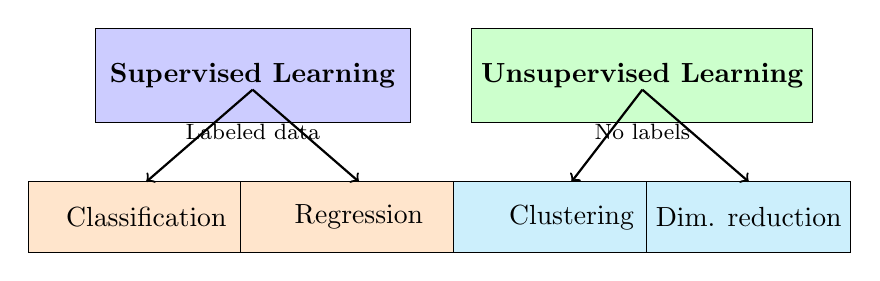
\begin{tikzpicture}[scale=0.9]
    \node[draw, rectangle, fill=blue!20, minimum width=4cm, minimum height=1.2cm] at (0,2) 
        {\textbf{Supervised Learning}};
    \node[text width=4cm, align=center, font=\footnotesize] at (0,1.2) 
        {Labeled data};
    
    \node[draw, rectangle, fill=green!20, minimum width=4cm, minimum height=1.2cm] at (5.5,2) 
        {\textbf{Unsupervised Learning}};
    \node[text width=4cm, align=center, font=\footnotesize] at (5.5,1.2) 
        {No labels};
    
    \node[draw, rectangle, fill=orange!20, minimum width=3cm, minimum height=0.9cm] at (-1.5,0) 
        {Classification};
    \node[draw, rectangle, fill=orange!20, minimum width=3cm, minimum height=0.9cm] at (1.5,0) 
        {Regression};
    
    \node[draw, rectangle, fill=cyan!20, minimum width=3cm, minimum height=0.9cm] at (4.5,0) 
        {Clustering};
    \node[draw, rectangle, fill=cyan!20, minimum width=2.5cm, minimum height=0.9cm] at (7,0) 
        {Dim. reduction};
    
    \draw[->, thick] (0,1.8) -- (-1.5,0.5);
    \draw[->, thick] (0,1.8) -- (1.5,0.5);
    \draw[->, thick] (5.5,1.8) -- (4.5,0.5);
    \draw[->, thick] (5.5,1.8) -- (7,0.5);
\end{tikzpicture}
\end{center}

\vspace{0.3cm}
\begin{block}{Today}
We focus on \alert{Classification}
\end{block}
\end{frame}

\begin{frame}{Classification: Definition}
\begin{block}{What is classification?}
Classification consists of \textbf{predicting a category} (class) for new observations, based on labeled examples.
\end{block}

\vspace{0.5cm}
\begin{columns}[T]
\column{0.48\textwidth}
\textbf{Input (Features):}
\begin{itemize}
    \item Measurable characteristics
    \item Descriptive variables
    \item Example: size, weight, color...
\end{itemize}

\column{0.48\textwidth}
\textbf{Output (Class):}
\begin{itemize}
    \item Predicted category
    \item Discrete variable
    \item Example: cat, dog, bird
\end{itemize}
\end{columns}
\end{frame}

\begin{frame}{Classification Examples}
\begin{center}
\begin{tabular}{|p{3.5cm}|p{4cm}|p{3cm}|}
\hline
\textbf{Application} & \textbf{Features (X)} & \textbf{Classes (y)} \\
\hline
Email spam & Words, sender, links & Spam / Not spam \\
\hline
Medical diagnosis & Symptoms, test results & Sick / Healthy \\
\hline
Image recognition & Image pixels & Cat / Dog / Bird \\
\hline
Bank credit & Income, age, history & Approved / Denied \\
\hline
Sentiment analysis & Text of a review & Positive / Negative / Neutral \\
\hline
Flower recognition & Sepal/petal size & Setosa / Versicolor / Virginica \\
\hline
\end{tabular}
\end{center}

\vspace{0.3cm}
\textit{Classification is everywhere!}
\end{frame}

\begin{frame}{Binary vs Multi-class Classification}
\begin{columns}[T]
\column{0.48\textwidth}
\begin{block}{Binary Classification}
\textbf{Only 2 classes}
\begin{itemize}
    \item Yes / No
    \item Spam / Ham
    \item Sick / Healthy
    \item Positive / Negative
\end{itemize}
\end{block}

\column{0.48\textwidth}
\begin{block}{Multi-class Classification}
\textbf{More than 2 classes}
\begin{itemize}
    \item 3 types of Iris flowers
    \item 10 digits (0-9)
    \item 26 letters (A-Z)
    \item 1000 object categories
\end{itemize}
\end{block}
\end{columns}

\vspace{0.5cm}
\begin{alertblock}{Important}
Today, we'll see algorithms that work for both!
\end{alertblock}
\end{frame}

\begin{frame}{The Classification Process}
\begin{center}
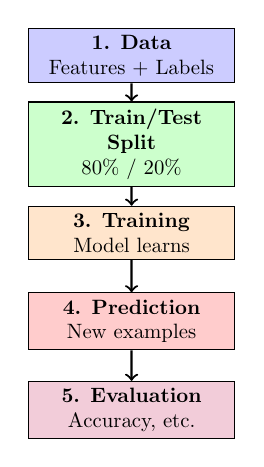
\begin{tikzpicture}[node distance=1.5cm, scale=0.75, every node/.style={scale=0.75}]
    \node[draw, rectangle, fill=blue!20, minimum width=3.5cm, text width=3cm, align=center] (data) 
        {\textbf{1. Data}\\ Features + Labels};
    
    \node[draw, rectangle, fill=green!20, minimum width=3.5cm, text width=3cm, align=center, below of=data] (split) 
        {\textbf{2. Train/Test Split}\\ 80\% / 20\%};
    
    \node[draw, rectangle, fill=orange!20, minimum width=3.5cm, text width=3cm, align=center, below of=split] (train) 
        {\textbf{3. Training}\\ Model learns};
    
    \node[draw, rectangle, fill=red!20, minimum width=3.5cm, text width=3cm, align=center, below of=train] (predict) 
        {\textbf{4. Prediction}\\ New examples};
    
    \node[draw, rectangle, fill=purple!20, minimum width=3.5cm, text width=3cm, align=center, below of=predict] (eval) 
        {\textbf{5. Evaluation}\\ Accuracy, etc.};
    
    \draw[->, thick] (data) -- (split);
    \draw[->, thick] (split) -- (train);
    \draw[->, thick] (train) -- (predict);
    \draw[->, thick] (predict) -- (eval);
\end{tikzpicture}
\end{center}
\end{frame}

%% ========== SECTION 2 ==========
\section{K-Nearest Neighbors (KNN)}

\begin{frame}{KNN: The Simplest Algorithm}
\begin{block}{Core Idea}
\textbf{``Tell me who your neighbors are, and I'll tell you who you are''}
\end{block}

\vspace{0.5cm}
\begin{columns}[T]
\column{0.48\textwidth}
\textbf{Principle:}
\begin{enumerate}
    \item Find the K nearest neighbors
    \item Look at their class
    \item Majority vote
    \item Assign the winning class
\end{enumerate}

\column{0.48\textwidth}
\begin{center}
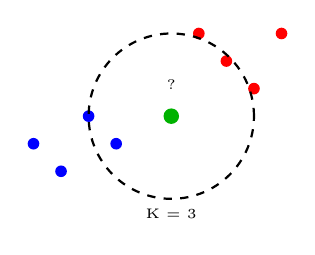
\begin{tikzpicture}[scale=0.7]
    % Blue points (class 1)
    \fill[blue] (1,1) circle (3pt);
    \fill[blue] (1.5,2) circle (3pt);
    \fill[blue] (0.5,1.5) circle (3pt);
    \fill[blue] (2,1.5) circle (3pt);
    
    % Red points (class 2)
    \fill[red] (4,3) circle (3pt);
    \fill[red] (4.5,2.5) circle (3pt);
    \fill[red] (5,3.5) circle (3pt);
    \fill[red] (3.5,3.5) circle (3pt);
    
    % Point to classify (green)
    \fill[green!70!black] (3,2) circle (4pt);
    \node[above, font=\tiny] at (3,2.3) {?};
    
    % K=3 circle
    \draw[dashed, thick] (3,2) circle (1.5);
    \node[below, font=\tiny] at (3,0.5) {K = 3};
\end{tikzpicture}
\end{center}
\end{columns}
\end{frame}

\begin{frame}{KNN: How Does It Work? (1/2)}
\begin{block}{Step 1: Compute the Distance}
For each point in the dataset, compute its distance to the new point.
\end{block}

\vspace{0.3cm}
\textbf{Euclidean distance (most common):}
\begin{center}
\Large
$d = \sqrt{(x_2-x_1)^2 + (y_2-y_1)^2}$
\end{center}

\vspace{0.3cm}
\begin{exampleblock}{Example}
Point A = (1, 2) and Point B = (4, 6)\\
$d = \sqrt{(4-1)^2 + (6-2)^2} = \sqrt{9 + 16} = \sqrt{25} = 5$
\end{exampleblock}
\end{frame}

\begin{frame}{KNN: How Does It Work? (2/2)}
\begin{block}{Step 2: Sort by Distance}
Keep the K closest points
\end{block}

\begin{block}{Step 3: Majority Vote}
Count the classes among the K neighbors
\end{block}

\begin{exampleblock}{Example with K=5}
\begin{itemize}
    \item Neighbor 1: Class A (distance: 1.2)
    \item Neighbor 2: Class A (distance: 1.5)
    \item Neighbor 3: Class B (distance: 1.8)
    \item Neighbor 4: Class A (distance: 2.1)
    \item Neighbor 5: Class B (distance: 2.3)
\end{itemize}
\textbf{Vote:} A=3, B=2 → \alert{Predicted class = A}
\end{exampleblock}
\end{frame}

\begin{frame}{The Parameter K: Impact}
\begin{center}
\includegraphics[width=0.95\textwidth]{knn_comparison.png}
\end{center}

\vspace{0.3cm}
\begin{alertblock}{Advice}
\begin{itemize}
    \item K too small → overfitting (noise)
    \item K too large → underfitting (loses detail)
    \item Common values: K = 3, 5, 7 (odd numbers to avoid ties)
\end{itemize}
\end{alertblock}
\end{frame}

\begin{frame}[fragile]{KNN with Scikit-learn}
\begin{lstlisting}
from sklearn.datasets import load_iris
from sklearn.model_selection import train_test_split
from sklearn.neighbors import KNeighborsClassifier
from sklearn.metrics import accuracy_score

# 1. Load the data
iris = load_iris()
X = iris.data
y = iris.target

# 2. Train/Test split
X_train, X_test, y_train, y_test = train_test_split(
    X, y, test_size=0.3, random_state=42)

# 3. Create the KNN model
knn = KNeighborsClassifier(n_neighbors=5)

# 4. Train
knn.fit(X_train, y_train)

# 5. Predict
y_pred = knn.predict(X_test)

# 6. Evaluate
accuracy = accuracy_score(y_test, y_pred)
print(f"Accuracy: {accuracy*100:.2f}%")
\end{lstlisting}
\end{frame}

\begin{frame}{KNN: Advantages and Disadvantages}
\begin{columns}[T]
\column{0.48\textwidth}
\begin{block}{Advantages ✓}
\begin{itemize}
    \item Simple to understand
    \item No training step
    \item Works well for small datasets
    \item No assumptions about the data
    \item Naturally multi-class
\end{itemize}
\end{block}

\column{0.48\textwidth}
\begin{block}{Disadvantages ✗}
\begin{itemize}
    \item Slow for large datasets
    \item Sensitive to un-normalized features
    \item Sensitive to noise
    \item Need to choose K
    \item Memory-intensive
\end{itemize}
\end{block}
\end{columns}

\vspace{0.5cm}
\begin{alertblock}{When to Use KNN?}
Small datasets, few features, need for simplicity
\end{alertblock}
\end{frame}

%% ========== SECTION 3 ==========
\section{Decision Trees}

\begin{frame}{Decision Trees: Intuition}
\begin{block}{The Idea}
A decision tree asks a series of \textbf{questions} about the features to arrive at a decision.
\end{block}

\vspace{0.3cm}
\begin{center}
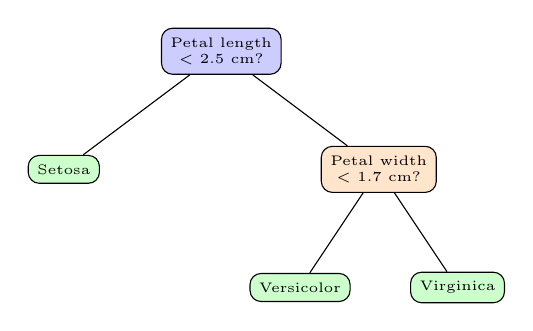
\begin{tikzpicture}[
    level distance=1.5cm,
    level 1/.style={sibling distance=4cm},
    level 2/.style={sibling distance=2cm},
    every node/.style={draw, rectangle, rounded corners, font=\tiny, align=center}
]
\node[fill=blue!20] {Petal length\\< 2.5 cm?}
    child {node[fill=green!20] {Setosa}}
    child {node[fill=orange!20] {Petal width\\< 1.7 cm?}
        child {node[fill=green!20] {Versicolor}}
        child {node[fill=green!20] {Virginica}}
    };
\end{tikzpicture}
\end{center}

\vspace{0.3cm}
\textit{Like a decision flowchart!}
\end{frame}

\begin{frame}{How Do We Build a Tree?}
\begin{block}{Algorithm (simplified)}
\begin{enumerate}
    \item Choose the best question to ask
    \item Split the data according to that question
    \item Repeat for each branch
    \item Stop when:
    \begin{itemize}
        \item All examples belong to the same class
        \item Maximum depth is reached
        \item Minimum number of examples is reached
    \end{itemize}
\end{enumerate}
\end{block}

\vspace{0.3cm}
\begin{alertblock}{Key Question}
How do we choose the \textbf{best} question?\\
→ The one that best separates the classes
\end{alertblock}
\end{frame}

\begin{frame}{Split Criterion: Gini and Entropy}
\begin{block}{Impurity Measures}
We want \textbf{pure} groups (a single class per group)
\end{block}

\vspace{0.3cm}
\begin{columns}[T]
\column{0.48\textwidth}
\textbf{Gini Index:}
\begin{center}
$Gini = 1 - \sum_{i=1}^{n} p_i^2$
\end{center}
\begin{itemize}
    \item Gini = 0 → perfectly pure
    \item Gini = 0.5 → 50/50 mix
\end{itemize}

\column{0.48\textwidth}
\textbf{Entropy:}
\begin{center}
$H = -\sum_{i=1}^{n} p_i \log_2(p_i)$
\end{center}
\begin{itemize}
    \item H = 0 → perfectly pure
    \item High H → disorder
\end{itemize}
\end{columns}

\vspace{0.4cm}
\begin{exampleblock}{Example}
Group with 10 blue and 0 red → Gini = 0 (pure!)\\
Group with 5 blue and 5 red → Gini = 0.5 (impure)
\end{exampleblock}
\end{frame}

\begin{frame}{Visual Example: Iris Dataset}
\begin{center}
\includegraphics[width=0.95\textwidth]{iris_2d_visualization.png}
\end{center}
\vspace{0.2cm}
\small
Petals separate the 3 species better than sepals!
\end{frame}

\begin{frame}{Decision Boundaries: KNN vs Tree}
\begin{center}
\includegraphics[width=0.95\textwidth]{decision_boundaries.png}
\end{center}
\vspace{0.2cm}
\small
\textbf{KNN:} Smooth boundaries | \textbf{Tree:} Rectangular boundaries
\end{frame}

\begin{frame}[fragile]{Decision Trees with Scikit-learn}
\begin{lstlisting}
from sklearn.tree import DecisionTreeClassifier
from sklearn.datasets import load_iris
from sklearn.model_selection import train_test_split
from sklearn.metrics import accuracy_score

# 1. Load the data
iris = load_iris()
X = iris.data
y = iris.target

# 2. Train/Test split
X_train, X_test, y_train, y_test = train_test_split(
    X, y, test_size=0.3, random_state=42)

# 3. Create the decision tree
tree = DecisionTreeClassifier(
    max_depth=3,        # Maximum depth
    min_samples_split=2 # Min examples to split
)

# 4. Train
tree.fit(X_train, y_train)

# 5. Predict
y_pred = tree.predict(X_test)

# 6. Evaluate
accuracy = accuracy_score(y_test, y_pred)
print(f"Accuracy: {accuracy*100:.2f}%")
\end{lstlisting}
\end{frame}

\begin{frame}{Important Parameters}
\begin{block}{Controlling Tree Complexity}
\begin{itemize}
    \item \textbf{max\_depth}: Maximum depth of the tree
    \begin{itemize}
        \item Too large → overfitting
        \item Too small → underfitting
    \end{itemize}
    
    \item \textbf{min\_samples\_split}: Minimum number of examples to split a node
    \begin{itemize}
        \item Larger → simpler tree
    \end{itemize}
    
    \item \textbf{min\_samples\_leaf}: Minimum number of examples in a leaf
    \begin{itemize}
        \item Avoids leaves with too little data
    \end{itemize}
    
    \item \textbf{criterion}: 'gini' or 'entropy'
    \begin{itemize}
        \item In practice, little difference
    \end{itemize}
\end{itemize}
\end{block}
\end{frame}

\begin{frame}{Trees: Advantages and Disadvantages}
\begin{columns}[T]
\column{0.48\textwidth}
\begin{block}{Advantages ✓}
\begin{itemize}
    \item Easy to understand and visualize
    \item No need for normalization
    \item Handles numeric and categorical features
    \item Handles missing values
    \item Fast to train and predict
    \item Shows feature importance
\end{itemize}
\end{block}

\column{0.48\textwidth}
\begin{block}{Disadvantages ✗}
\begin{itemize}
    \item Tendency to overfit
    \item Unstable (small changes → different tree)
    \item Bias toward dominant features
    \item Less accurate than other methods
\end{itemize}
\end{block}
\end{columns}

\vspace{0.5cm}
\begin{alertblock}{Solution}
\textbf{Random Forests} (next class) combine several trees to be more robust!
\end{alertblock}
\end{frame}

%% ========== SECTION 4 ==========
\section{Evaluation Metrics}

\begin{frame}{Why Evaluate?}
\begin{block}{Fundamental Question}
How do we know if our model is \textbf{good}?
\end{block}

\vspace{0.5cm}
\begin{alertblock}{Golden Rule}
\textbf{NEVER} evaluate on the training data!\\
→ Risk of overestimating performance
\end{alertblock}

\vspace{0.5cm}
\begin{center}
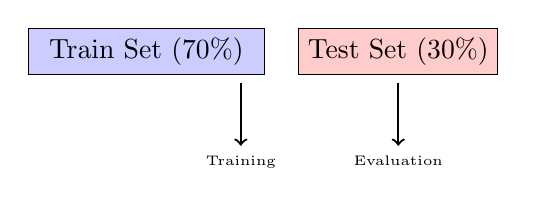
\begin{tikzpicture}[scale=0.8]
    \node[draw, rectangle, fill=blue!20, minimum width=3cm] at (0,0) {Train Set (70\%)};
    \node[draw, rectangle, fill=red!20, minimum width=2cm] at (4,0) {Test Set (30\%)};
    
    \draw[->, thick] (1.5,-0.5) -- (1.5,-1.5) node[below, text width=2.5cm, align=center, font=\tiny] 
        {Training};
    \draw[->, thick] (4,-0.5) -- (4,-1.5) node[below, text width=2.5cm, align=center, font=\tiny] 
        {Evaluation};
\end{tikzpicture}
\end{center}
\end{frame}

\begin{frame}{Accuracy}
\begin{block}{Definition}
Percentage of correct predictions
\end{block}

\begin{center}
\Large
$Accuracy = \frac{\text{Number of correct predictions}}{\text{Total number of predictions}}$
\end{center}

\vspace{0.3cm}
\begin{exampleblock}{Example}
Out of 100 flowers:
\begin{itemize}
    \item 95 correctly classified
    \item 5 misclassified
\end{itemize}
$Accuracy = \frac{95}{100} = 0.95 = 95\%$
\end{exampleblock}

\vspace{0.3cm}
\begin{alertblock}{Warning!}
Accuracy can be misleading if classes are imbalanced!
\end{alertblock}
\end{frame}

\begin{frame}{The Problem of Imbalanced Classes}
\begin{exampleblock}{Example: Fraud Detection}
Dataset: 1000 transactions
\begin{itemize}
    \item 990 normal
    \item 10 fraudulent
\end{itemize}

\vspace{0.3cm}
\textbf{Naive model:} Predict "Normal" for everything\\
→ Accuracy = 99\%!

\vspace{0.3cm}
\textbf{But:} 0\% of fraud detected!
\end{exampleblock}

\vspace{0.3cm}
\begin{alertblock}{Solution}
Use other metrics: Precision, Recall, F1-Score
\end{alertblock}
\end{frame}

\begin{frame}{Confusion Matrix}
\begin{block}{Definition}
A table showing predictions vs actual values
\end{block}

\vspace{0.3cm}
\begin{center}
\begin{tabular}{cc|c|c|}
\multicolumn{2}{c}{} & \multicolumn{2}{c}{\textbf{Prediction}} \\
\cline{3-4}
\multicolumn{2}{c|}{} & Positive & Negative \\
\hline
\multirow{\textbf{Actual}} 
& Positive & TP & FN \\
\cline{2-4}
& Negative &  FP &  TN \\
\hline
\end{tabular}
\end{center}

\vspace{0.3cm}
\begin{itemize}
    \item \textbf{TP} (True Positive): Predicted positive, correct
    \item \textbf{TN} (True Negative): Predicted negative, correct
    \item \textbf{FP} (False Positive): Predicted positive, wrong (Type I Error)
    \item \textbf{FN} (False Negative): Predicted negative, wrong (Type II Error)
\end{itemize}
\end{frame}

\begin{frame}{Confusion Matrix Example}
\begin{exampleblock}{Classifying 100 emails}
\begin{center}
\begin{tabular}{cc|c|c|c|}
\multicolumn{2}{c}{} & \multicolumn{2}{c}{\textbf{Prediction}} \\
\cline{3-4}
\multicolumn{2}{c|}{} & Spam & Ham \\
\hline
\multirow{\textbf{Actual}} 
& Spam & 35 &  5 \\
\cline{2-4}
& Ham &  3 &  57 \\
\hline
\end{tabular}
\end{center}

\vspace{0.3cm}
\begin{itemize}
    \item TP = 35 (spam correctly detected)
    \item TN = 57 (ham correctly classified)
    \item FP = 3 (ham classified as spam)
    \item FN = 5 (spam not detected)
\end{itemize}

\vspace{0.3cm}
$Accuracy = \frac{35 + 57}{100} = 92\%$
\end{exampleblock}
\end{frame}

\begin{frame}{Precision and Recall}
\begin{columns}[T]
\column{0.48\textwidth}
\begin{block}{Precision}
Among the positive predictions, how many are correct?
\end{block}

\begin{center}
$Precision = \frac{TP}{TP + FP}$
\end{center}

\textit{``When I say spam, is it really spam?''}

\column{0.48\textwidth}
\begin{block}{Recall}
Among the actual positives, how many are detected?
\end{block}

\begin{center}
$Recall = \frac{TP}{TP + FN}$
\end{center}

\textit{``Do I detect all the spam?''}
\end{columns}

\vspace{0.5cm}
\begin{exampleblock}{Previous Example}
$Precision = \frac{35}{35+3} = 0.92 = 92\%$\\
$Recall = \frac{35}{35+5} = 0.875 = 87.5\%$
\end{exampleblock}
\end{frame}

\begin{frame}{F1-Score}
\begin{block}{Problem}
Precision and Recall can conflict!
\end{block}

\begin{alertblock}{Trade-off}
\begin{itemize}
    \item Increasing Precision → decreases Recall
    \item Increasing Recall → decreases Precision
\end{itemize}
\end{alertblock}

\vspace{0.3cm}
\begin{block}{F1-Score: Harmonic Mean}
\begin{center}
\Large
$F1 = 2 \times \frac{Precision \times Recall}{Precision + Recall}$
\end{center}
\end{block}

\vspace{0.3cm}
\begin{itemize}
    \item F1-Score balances Precision and Recall
    \item Useful when classes are imbalanced
\end{itemize}
\end{frame}

\begin{frame}[fragile]{Computing Metrics with Scikit-learn}
\begin{lstlisting}
from sklearn.metrics import accuracy_score, precision_score, recall_score, f1_score
from sklearn.metrics import confusion_matrix, classification_report

# Predictions
y_pred = model.predict(X_test)

# Accuracy
accuracy = accuracy_score(y_test, y_pred)
print(f"Accuracy: {accuracy:.2f}")

# Precision, Recall, F1
precision = precision_score(y_test, y_pred, average='weighted')
recall = recall_score(y_test, y_pred, average='weighted')
f1 = f1_score(y_test, y_pred, average='weighted')

print(f"Precision: {precision:.2f}")
print(f"Recall: {recall:.2f}")
print(f"F1-Score: {f1:.2f}")

# Confusion matrix
cm = confusion_matrix(y_test, y_pred)
print(cm)

# Full report
print(classification_report(y_test, y_pred))
\end{lstlisting}
\end{frame}

\begin{frame}{Confusion Matrices: KNN vs Tree}
\begin{center}
\includegraphics[width=0.95\textwidth]{confusion_matrices.png}
\end{center}
\vspace{0.2cm}
\small
Both models achieve 100\% accuracy on the Iris test set!
\end{frame}

%% ========== SECTION 5 ==========
\section{Complete Practical Example}

\begin{frame}[fragile]{Iris Dataset: Reminder}
\begin{lstlisting}
from sklearn.datasets import load_iris
import pandas as pd

# Load
iris = load_iris()

# Create a DataFrame for visualization
df = pd.DataFrame(iris.data, columns=iris.feature_names)
df['species'] = iris.target

print(df.head())
print("\nClasses:", iris.target_names)
print("Features:", iris.feature_names)
\end{lstlisting}

\vspace{0.3cm}
\begin{itemize}
    \item 150 flowers
    \item 4 features (sepal/petal length and width)
    \item 3 classes (Setosa, Versicolor, Virginica)
\end{itemize}
\end{frame}

\begin{frame}[fragile]{KNN vs Tree Comparison (1/2)}
\begin{lstlisting}
from sklearn.datasets import load_iris
from sklearn.model_selection import train_test_split
from sklearn.neighbors import KNeighborsClassifier
from sklearn.tree import DecisionTreeClassifier
from sklearn.metrics import accuracy_score, classification_report

# Load and split
iris = load_iris()
X_train, X_test, y_train, y_test = train_test_split(
    iris.data, iris.target, test_size=0.3, random_state=42)

# KNN
knn = KNeighborsClassifier(n_neighbors=5)
knn.fit(X_train, y_train)
y_pred_knn = knn.predict(X_test)

# Decision Tree
tree = DecisionTreeClassifier(max_depth=3, random_state=42)
tree.fit(X_train, y_train)
y_pred_tree = tree.predict(X_test)
\end{lstlisting}
\end{frame}

\begin{frame}[fragile]{KNN vs Tree Comparison (2/2)}
\begin{lstlisting}
# Evaluate KNN
print("=== KNN ===")
print(f"Accuracy: {accuracy_score(y_test, y_pred_knn):.2f}")
print(classification_report(y_test, y_pred_knn, 
                            target_names=iris.target_names))

# Evaluate Tree
print("\n=== Decision Tree ===")
print(f"Accuracy: {accuracy_score(y_test, y_pred_tree):.2f}")
print(classification_report(y_test, y_pred_tree, 
                            target_names=iris.target_names))
\end{lstlisting}

\vspace{0.3cm}
\textbf{Typical results:}
\begin{itemize}
    \item KNN: 95-98\% accuracy
    \item Tree: 93-96\% accuracy
\end{itemize}
\end{frame}

\begin{frame}[fragile]{Visualizing the Decision Tree}
\begin{lstlisting}
from sklearn.tree import plot_tree
import matplotlib.pyplot as plt

# Create a large figure
plt.figure(figsize=(20,10))

# Visualize the tree
plot_tree(tree, 
          feature_names=iris.feature_names,
          class_names=iris.target_names,
          filled=True,
          rounded=True,
          fontsize=10)

plt.title("Decision Tree - Iris Dataset")
plt.savefig('decision_tree_iris.png', dpi=150, bbox_inches='tight')
plt.show()
\end{lstlisting}

\vspace{0.3cm}
\textit{Helps us understand how the tree makes its decisions!}
\end{frame}

\begin{frame}{The Visualized Decision Tree}
\begin{center}
\includegraphics[width=0.98\textwidth]{decision_tree_full.png}
\end{center}
\end{frame}

\begin{frame}[fragile]{Feature Importance}
\begin{columns}[T]
\column{0.45\textwidth}
\begin{lstlisting}
import numpy as np
import matplotlib.pyplot as plt

# Get importance values
importances = tree.feature_importances_
features = iris.feature_names

# Sort
indices = np.argsort(
    importances)[::-1]

# Visualize
plt.bar(range(len(importances)), 
        importances[indices])
plt.xticks(range(len(importances)), 
    [features[i] for i in indices])
plt.title("Feature Importance")
plt.show()
\end{lstlisting}

\column{0.53\textwidth}
\includegraphics[width=\textwidth]{feature_importance.png}
\end{columns}
\end{frame}

%% ========== SECTION 6 ==========
\section{Practical Advice}

\begin{frame}{KNN vs Trees: When to Use What?}
\begin{center}
\begin{tabular}{|p{5cm}|p{5cm}|}
\hline
\textbf{Use KNN if:} & \textbf{Use Trees if:} \\
\hline
Small/medium dataset & Medium/large dataset \\
\hline
Few features (< 20) & Many features \\
\hline
Well-normalized data & No need to normalize \\
\hline
Complex non-linear relationships & Need for interpretability \\
\hline
Training time not critical & Prediction time matters \\
\hline
No need for explanation & Need to understand the rules \\
\hline
\end{tabular}
\end{center}

\vspace{0.5cm}
\begin{alertblock}{In practice}
Try both and compare!
\end{alertblock}
\end{frame}

\begin{frame}{Final Comparison: Performance}
\begin{center}
\includegraphics[width=0.8\textwidth]{final_comparison.png}
\end{center}
\vspace{0.2cm}
\small
On Iris, both algorithms achieve excellent performance!
\end{frame}

\begin{frame}{Best Practices}
\begin{enumerate}
    \item \textbf{Always} split train/test
    \item \textbf{Normalize} the data for KNN
    \item \textbf{Test several values} of K (KNN) or max\_depth (Trees)
    \item \textbf{Visualize} the results (confusion matrix)
    \item \textbf{Don't} rely on accuracy alone
    \item \textbf{Check} for overfitting (train vs test accuracy)
    \item \textbf{Understand} the model's errors
\end{enumerate}

\vspace{0.5cm}
\begin{alertblock}{Recommended Workflow}
Exploration → Preparation → Several models → Comparison → Best model
\end{alertblock}
\end{frame}

\begin{frame}{Avoiding Overfitting}
\vspace{0.2cm}
\begin{columns}[T]
\column{0.48\textwidth}
\textbf{With KNN:}
\begin{itemize}
    \item Increase K
    \item Normalize the features
    \item Reduce the number of features
    \item More training data
\end{itemize}

\column{0.48\textwidth}
\textbf{With Trees:}
\begin{itemize}
    \item Limit max\_depth
    \item Increase min\_samples\_split
    \item Increase min\_samples\_leaf
    \item Pruning
\end{itemize}
\end{columns}

\begin{center}
\includegraphics[width=0.8\textwidth]{overfitting_analysis.png}
\end{center}
\end{frame}

\begin{frame}[fragile]{Practice Exercise}
\begin{block}{Your Turn!}
\begin{enumerate}
    \item Load the Iris dataset
    \item Explore the data (shape, describe, visualization)
    \item Split into train/test (70/30)
    \item Train a KNN with K=3
    \item Train a tree with max\_depth=3
    \item Compare both models (accuracy, confusion matrix)
    \item Test different values of K and max\_depth
    \item Find the best parameters
    \item Visualize the final tree
    \item Interpret the results
\end{enumerate}
\end{block}
\end{frame}

\begin{frame}{Recap}
\begin{block}{What You've Learned}
\begin{itemize}
    \item \textbf{Classification}: predicting categories
    \item \textbf{KNN}: vote of the K nearest neighbors
    \item \textbf{Decision trees}: a series of questions
    \item \textbf{Metrics}: accuracy, precision, recall, F1
    \item \textbf{Confusion matrix}: visualizing errors
    \item \textbf{Best practices}: normalization, validation, avoiding overfitting
\end{itemize}
\end{block}


\end{frame}



\end{document}
